\documentclass[10pt,twocolumn]{article}
\usepackage{geometry}
\geometry{verbose,headsep=3cm,tmargin=2.5cm,bmargin=2.5cm,lmargin=2.0cm,rmargin=2.0cm}
\usepackage{graphicx}
\usepackage{xcolor}
\usepackage[font=small]{caption}
\usepackage{amsmath,amssymb,latexsym}
\usepackage{marvosym}
\usepackage{url}
\usepackage{lipsum}
\usepackage{bm}
\usepackage{float}
\usepackage[english]{babel}
\usepackage{hyperref}
\usepackage{epsf}
\usepackage{float}
\usepackage{mathpazo}
\usepackage{pifont}
\usepackage{wrapfig}
\usepackage{multicol}
\usepackage{enumitem}
\usepackage{xcolor}
\usepackage{framed}
\usepackage[utf8]{inputenc}
% Document font:
\usepackage{charter}
\graphicspath{{DWGs/}}

\begin{document}

\twocolumn[{
\begin{@twocolumnfalse}

  \begin{center}
%\textcolor{lgray}
    \vskip-5em

    \hfill
    \fontsize{10}{10}\selectfont {\textit{Bruxelles, February 2019}}

    \vskip2ex
    
	\vspace{5ex}
	
    \fontsize{24}{10}\selectfont {Notes on Dynamic Mode Decomposition}
    
    \fontsize{18}{10}\selectfont {(with some code)}



  \noindent%
    
\vskip1ex

{\rule{\textwidth}{0.5pt}}

  \end{center}
  
    \fontsize{7}{10}\selectfont {This work is licensed under the Creative Commons Attribution-NonCommercial-ShareAlike 4.0 International (CC BY-NC-SA 4.0) license.}

\vspace{6mm}

\end{@twocolumnfalse}
}]

\setlength{\parindent}{0cm}

\vspace{10mm}

\setlength{\parindent}{0cm}

\fontsize{14}{10}\selectfont {Kamila Zdybał}

\vspace{2mm}

\fontsize{8}{10}\selectfont {\textit{Université libre de Bruxelles, kamila.zdybal@ulb.ac.be}}

\fontsize{8}{10}\selectfont {\textit{camillejr.github.io/science-docs, kamila.zdybal@gmail.com}}

\vspace{2mm}



\section*{Preface}

\textit{Dynamic Mode Decomposition} (DMD) is a data-driven method for approximating a generally nonlinear dynamical system with a linear one. It can be used for finding low-rank structures in multi-dimensional data sets, as well as predicting the future state of the system with inference made solely from the collected data.

This document is a combination of various content on DMD found on the internet. The first are two lectures on Dynamic Mode Decomposition: [\ref{bib:kutz_1}] and [\ref{bib:kutz_2}] by Prof. Nathan Kutz from the University of Washington. Other references are mentioned along the way.

\,\,

This document is still in preparation. Please feel free to contact me with any suggestions, corrections or comments.

\section*{Keywords}

\textit{Dynamic Mode Decomposition (DMD), linear algebra, matrix decomposition, matrix approximation, linear dynamical systems, complex plane}



\tableofcontents


\section{Setting the stage}

This small opening section is there to give you a bit of intuition for DMD, which will be complimentary in understanding the incoming mathematical formulation. It is assumed that you have some general idea about what it means to perform data decomposition.

The main purpose of DMD is to find \textit{dynamic modes} underlying the data set. The modes are \textit{dynamic} in a sense that they are spatial structures, each associated with a certain time evolution given by frequency of oscillations. In other words, in DMD we not only know how the system can be decomposed spatially (what spatial structures it is composed of), but also how each spatial structure behaves in time. The original data set can then be reconstructed by summing up the dynamic modes, or approximated by summing up a portion of the dynamic modes. 

\begin{figure}[H]
\centering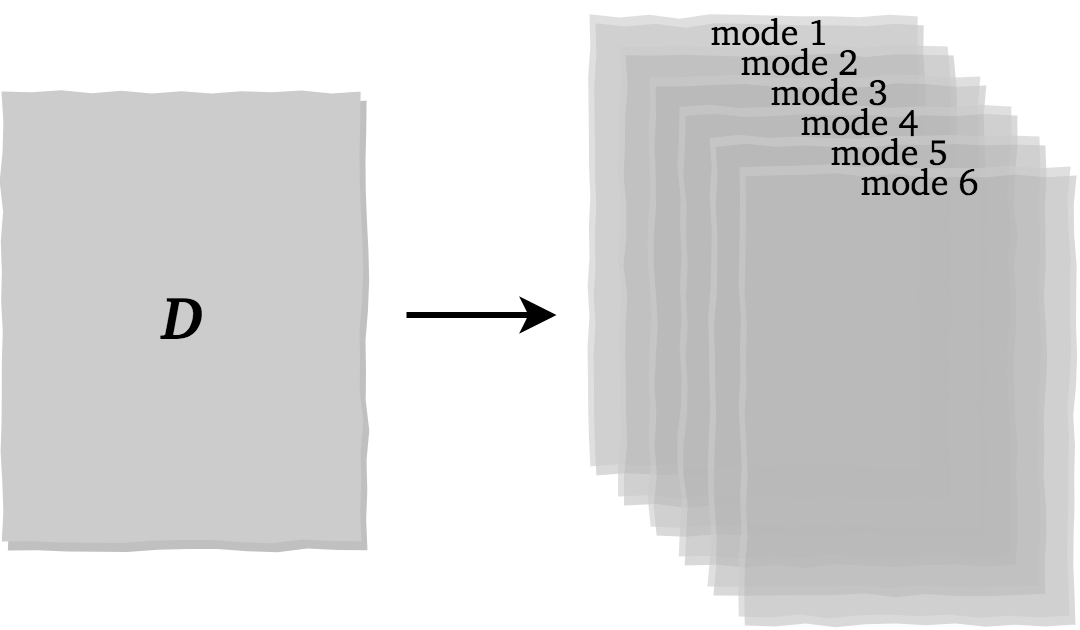
\includegraphics[width=5.5cm]{DMD-modal-decomposition.png}
\caption{Modal decomposition of a data matrix $\bm{D}$.}
\label{fig:modal-decomposition}
\end{figure}

In addition to the original data being reconstructed from its modes, different data decomposition methods will give a different meaning to the modes themselves. In general, we would like the modes to have a meaningful physical interpretation, as that will allow to extract additional information about the physics of the original data set.

\subsection{DMD of a flipbook}

To take a pictorial example, we may think of DMD as designing a flipbook [\ref{bib:andymation}]. However, every page of a flipbook is not a DMD mode. Rather, each mode is such element of all the flipbook pages which has got the same behaviour in time.

Let's say that each slide is composed of a background which is the same in every slide (it is constant in time). There might also be an animation of moving objects happening in the foreground where some parts are animated as moving faster and some as moving slowly.

We associate a certain number, say $\lambda$, to describe the evolution in time of every separate element (spatial structure) of the animation. This number will have a meaning of frequency of appearance.

And hence the background might be thought of as one spatial mode that has got a a constant time behaviour - it is present on every flipbook page. A ball bouncing on the foreground might be another mode, associated with its $\lambda$. 

The analogy presented in this section is based on \cite{Grosek}.

\section{Dynamical systems}

Dynamic Mode Decomposition connects strongly with the arguments made for \textit{dynamical systems} - systems that change in time. There is an interesting intuition carried from one-dimensional linear dynamical systems to multi-dimensional linear dynamical systems which we will briefly present here. For a more thorough explanation the reader is encouraged to look into \cite{Prof_Edward_Scheinerman}. 

Introducing the dynamical systems will be a good tool to understand the underlying concepts of DMD, especially the role of eigendecomposition which will appear as we present the theory in section \ref{sec:theory}.

\subsection{One-dimensional linear dynamical system}


\subsection{Multi-dimensional linear dynamical system}


\section{Description of a dynamical system}

We have a system described by a differential equation:

\begin{equation} \label{eq:system_DE}
\frac{d \vec{\bm{x}}(t)}{dt} = f(\vec{\bm{x}}, t, \text{varargin})
\end{equation}

where the function $f(\vec{\bm{x}}, t, \text{varargin})$ is a way of \textit{modeling} that system.

We also have collected \textit{measurements} of the system at different points in space at time $k$, in the form of a vector(s) $\vec{\bm{y}}_k$:

\begin{equation}
\vec{\bm{y}}_k = g(\vec{x}_k)
\end{equation}

\begin{wrapfigure}{R}{0.2\textwidth}
\centering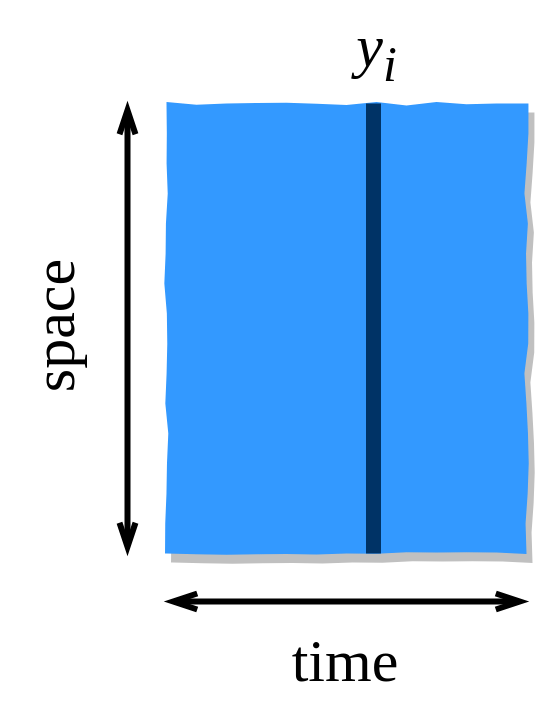
\includegraphics[width=3.5cm]{data-matrix.png}
\caption{Data matrix with measurements of the system.}
\label{fig:data-matrix}
\end{wrapfigure}

where $\vec{x}_k$ is the quantity of interest that we are aiming at measuring. The fact that we might not be able to measure it directly is accounted for by some function $g()$ (although it might happen that $\vec{y}_k = \vec{x}_k$, meaning that we are able to measure $\vec{x}_k$ directly).

Notice, that for measurements at many moments in time, we may stack all the collected vectors $\vec{y}_i$ for different times $i$ to create a matrix whose columns represent time snapshots and whose rows represent position in space - see Figure \ref{fig:data-matrix}. This is a matrix that we are going to work with.

\subsection{Linearizing the nonlinear dynamical systems}

We are from now interested in systems where the governing equation from eq.(\ref{eq:system_DE}) is not known (in other words, the function $f$ is unknown) and we solely rely on measurements of the system which, in general, form a high-dimensional data set.

In the Dynamic Mode Decomposition we approximate that data set by a linear dynamical system of the form:

\begin{equation} \label{eq:system_linear}
\frac{d \vec{x}(t)}{dt} = \bm{A} \vec{x}(t)
\end{equation}

This is in fact a very handy approximation since we are able to write down exact solutions to linear systems.

Once we assume that the general solution is of the form:

\begin{equation} \label{eq:general_solution}
\vec{x}(t) = \vec{v} e^{\bm{\lambda} t}
\end{equation}

to obtain the parameters we effectively solve the eigenvalue problem:

\begin{equation} \label{eq:eigenvalue_solution}
\bm{A} \vec{v} = \bm{\lambda} \vec{v}
\end{equation}

The exact solution to the linear system from eq.(\ref{eq:system_linear}) is:

\begin{equation} \label{eq:soln_exact}
x = \sum_{j = 1}^{n} b_j \phi_j e^{\lambda_j t}
\end{equation}

For a reader interested in how this solution was derived, more can be found in appendix \ref{app:A}. 

\section{Dynamic Mode Decomposition theory}\label{sec:theory}

\subsection{Exact DMD}

For the moment, we assume that we can measure the system directly, that is we measure $\vec{y}_i = \vec{x}_i$. Moreover, we assume that our data is collected in equal\footnote{Which is indeed a special case for real life measurements. Check section \ref{sec:view} for more information.} time steps $\Delta t$. The measurements are combined inside a large matrix $\bm{X}$ where each of its columns represents one time snapshot:

\begin{equation} \label{eq:X}
\bm{X} = 
\begin{bmatrix}
    \vec{x}_1 & \vec{x}_2 & \vec{x}_3 & \dots & \vec{x}_{m}
\end{bmatrix}
\end{equation}

We split the large matrix $\bm{X}$ into two matrices $\bm{X_1}$ and $\bm{X_2}$ such that:

\begin{equation} \label{eq:X1}
\bm{X_1} = 
\begin{bmatrix}
    \vec{x}_1 & \vec{x}_2 & \vec{x}_3 & \dots & \vec{x}_{m-1}
\end{bmatrix}
\end{equation}

\begin{equation} \label{eq:X2}
\bm{X_2} = 
\begin{bmatrix}
    \vec{x}_2 & \vec{x}_3 & \vec{x}_4 & \dots & \vec{x}_{m}
\end{bmatrix}
\end{equation}

If we now assume that a linear operator will map the first element of $\bm{X_1}$ with the first element of $\bm{X_2}$, second with the second, third with the third, and so on, matrix $\bm{X_2}$ can be thought of as a matrix representing the \textit{future state} of the matrix $\bm{X_1}$. That linear operator is assumed to be a matrix $\bm{A}$. 

\begin{figure}[H]
\centering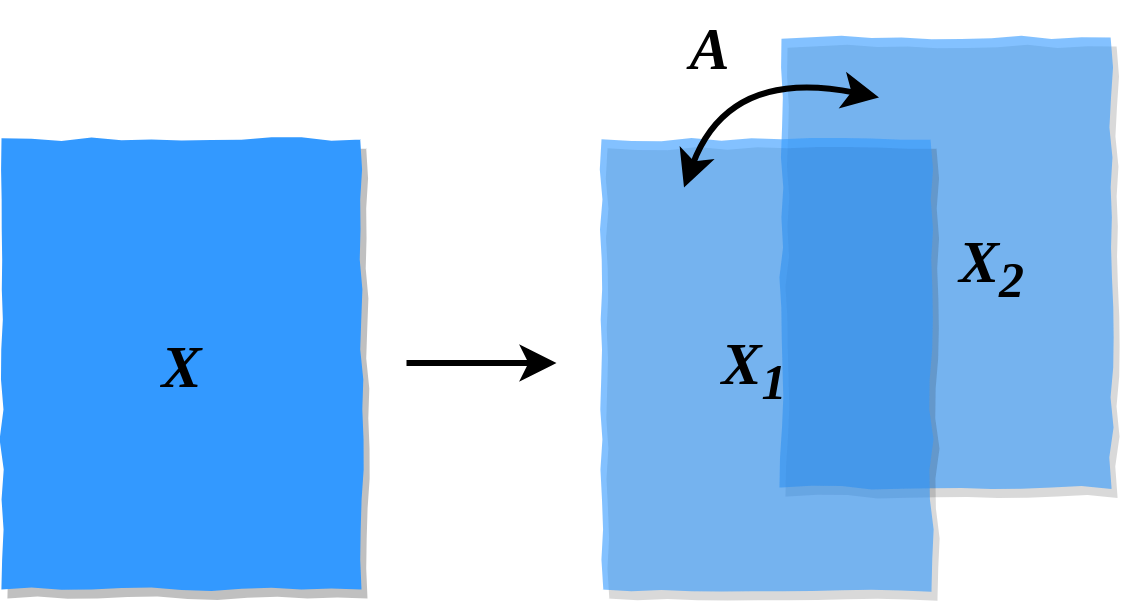
\includegraphics[width=5.5cm]{data-split.png}
\caption{Splitting the data matrix into \textit{past} and \textit{future} matrices $\bm{X_1}$ and $\bm{X_2}$, linked by the linear operator $\bm{A}$.}
\label{fig:linear_system}
\end{figure}

Note here, that for nonlinear systems, a matrix that transforms $\vec{x}_1$ to $\vec{x}_2$ is different from a matrix that transforms $\vec{x}_2$ to $\vec{x}_3$ and so on. DMD assumes, however, that there is one matrix $\bm{A}$ that does all these transformations at once, with the least amount of error. It finds the \textit{best-fit} linear dynamical system for the non-linear data set. In mathematical terms, we are looking for such $\bm{A}$ that:

\begin{equation} \label{eq:linear_dynamics}
\bm{X_2} = \bm{A} \bm{X_1}
\end{equation}

To solve such system we multiply both sides by the \textit{pseudo-inverse} of matrix $\bm{X_1}$ which we denote by $\bm{X_1}^{+}$:

\begin{equation} \label{eq:linear_dynamics_A}
\bm{A} = \bm{X_2} \bm{X_1}^{+}
\end{equation}

The pseudo-inverse described here, also known as the Moore-Penrose inverse\footnote{Check appendix \ref{app:B} for more information.}, is computed using the least squares method. There is therefore certain information lost when going from eq.(\ref{eq:linear_dynamics}) to eq.(\ref{eq:linear_dynamics_A}).

Once we have solved for matrix $\bm{A}$, we can go back to eq.(\ref{eq:eigenvalue_solution}) and solve for eigenvalues and eigenvectors.

Up to this point, this is what the \textbf{exact DMD} computes. There is however a problem that the eq.(\ref{eq:linear_dynamics_A}) may pose when numerics are involved and this will be addressed in the next section. 

\subsection{Going low-rank}

Matrices $\bm{X_1}^{+}$ and $\bm{X_2}$ typically represent huge spacial dimensionality\footnote{This is often the case for data sets where we have very few snapshots in time but a large number of spacial points where the measurements were taken. Graphically, we might think of those matrices as being "tall" and this is illustrated in Figure \ref{fig:data-matrix}.} which in turn means that the matrix $\bm{A}$ can become a square matrix of a massive size. 

\begin{wrapfigure}{R}{0.2\textwidth}
\centering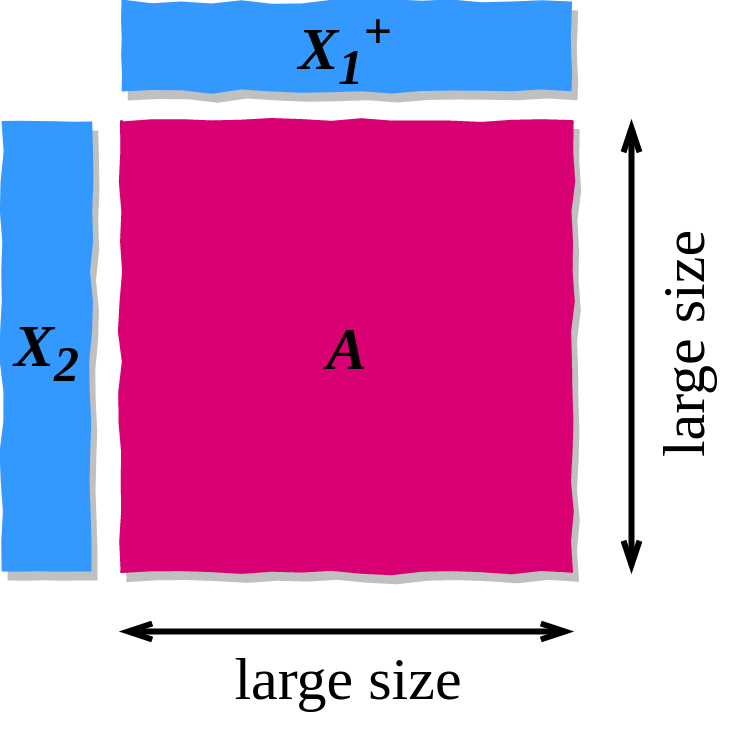
\includegraphics[width=3.5cm]{getting-A.png}
\caption{Building the linear operator $\bm{A}$ in exact DMD.}
\label{fig:building-A}
\end{wrapfigure}

We are hence reluctant to perform the multiplication of matrices as is stated in eq.(\ref{eq:linear_dynamics_A}). 

The hope comes from the \textit{Singular Value Decomposition} (SVD). We belive that there are low-rank structures hidden in the data set and we are able to reduce the dimensionality of matrix $\bm{A}$ without significant loss of information\footnote{Professor Kutz said a very interesting sentence here, that the multiplication presented in Figure \ref{fig:building-A} completely ignores the fact that there might be low-rank structures in our data set.}.

We perform the SVD on matrix $\bm{X_1}$ and decompose it to the component matrices: $\bm{U}$, $\bm{\Sigma}$ and $\bm{V}$.

\begin{equation} \label{eq:solution}
\bm{X_1} = \bm{U} \bm{\Sigma} \bm{V}^T 
\end{equation}

Based on the rank structure of the matrix $\bm{X_1}$ (one way to get information about the rank structure is to plot the elements from the diagonal of the matrix $\bm{\Sigma}$) we perform a rank-$r$ truncation on the SVD decomposition and approximate the matrix $\bm{X_1}$ by its low-rank (rank-$r$) representation:

\begin{equation} \label{eq:solution-approx}
\bm{X_1} \approx \bm{X_{1r}} = \bm{U_r} \bm{\Sigma_r} \bm{V_r}^T 
\end{equation}

The pseudo-inverse of the truncated matrix is:

\begin{equation} \label{eq:pseudo-inverse}
\bm{X_{1r}}^{+} = \bm{V_r}  \bm{\Sigma_r}^{-1} \bm{U_r}^T
\end{equation}

The usefulness of this decomposition might not yet be evident, since the matrix $\bm{X_{1r}}$ is of the same size as matrix $\bm{X_{1}}$, they only differ by rank. The idea is to nevertheless use the SVD decomposition but also, to generate a matrix similar to the matrix $\bm{A}$ (since similar matrices share eigenvalues and eigenvectors, among some other properties) but one that will have a smaller size (in fact, it will be size $(r \times r)$). This similar matrix will be denoted $\underline{\bm{A}}$. Since it has a lower size than the original matrix $\bm{A}$, we will only retrieve $r$ eigenvectors and eigenvalues.

\begin{wrapfigure}{R}{0.25\textwidth}
\centering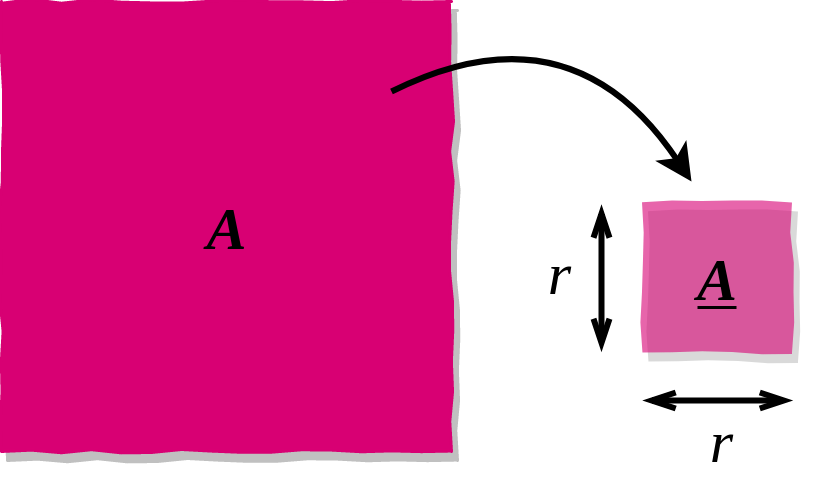
\includegraphics[width=4cm]{similar-matrices.png}
\caption{Similarity transform of matrix $\bm{A}$ to reduce its size.}
\label{fig:similar-matrices}
\end{wrapfigure}

What will now follow are clever mathematical steps performed to avoid computation of the large matrix $\bm{A}$.

We come back to the eq.(\ref{eq:linear_dynamics_A}) and

We perform a \textit{similarity transform} of the matrix $\bm{A}$:

\begin{equation} \label{eq:similarity-transform}
\underline{\bm{A}} = \bm{U_r}^T \bm{A} \bm{U_r}
\end{equation}

Matrix $\bm{A}$ can be written as:

\begin{equation} \label{eq:A}
\bm{A} = \bm{X_2} \bm{V_r} \bm{\Sigma_r}^{-1} \bm{U_r}^T
\end{equation}

The similar matrix $\underline{\bm{A}}$ can be written as:

\begin{equation} \label{eq:A_underline}
\underline{\bm{A}} = \bm{U_r}^T \bm{X_2} \bm{V_r} \bm{\Sigma_r}^{-1} 
\end{equation}

taking into account that $\bm{U_r}^T \bm{U_r} = \bm{I}$.

We have thus chosen a low-dimensional subspace by performing rank-$r$ truncation in which we now find the solution to the linear dynamical system presented initially. The solution is built in this low-dimensional subspace.

\subsection{Eigendecomposition}

Now that we have computed the similar matrix $\underline{\bm{A}}$, we move on to perform the eigendecomposition:

\begin{equation} \label{eq:A_underline}
[\bm{W}, \bm{\Lambda}] = \text{eig}(\underline{\bm{A}})
\end{equation}

The matrix $\bm{W}$ is a matrix whose columns are the eigenvectors of $\underline{\bm{A}}$. The matrix $\bm{\Lambda}$ is a diagonal matrix of eigenvalues $\lambda_i$ which, in the most general case, are complex numbers. We have therefore obtained "coupled" quantities - each eigenvector has got its corresponding eigenvalue - and that link is exploited by the Dynamic Mode Decomposition to give a physical meaning to eigenvectors and eigenvalues.

The eigenvectors will form the spacial modes of DMD. 

We can write the complex eigenvalue as:

\begin{equation} \label{eq:A_underline}
\lambda_i = e^{(\sigma_i + i \omega_i) \Delta t} 
\end{equation}

The real part of the eigenvalue corresponds to the growth rate of that particular mode and the imaginary part represents the oscillatory frequency of a mode.

\subsection{Going back to the original dimensions}

In the previous section we have retrieved $r$ eigenvalues and eigenvectors but our original dimension for the propagator matrix was $n_t$. We have reduced the dimensionality of the problem but our final solution will only make sense to us if it is expressed in $n_t$ dimensions.
Once the model has been built in the low-dimensional subspace, we want to move to the original dimensions. 

The DMD modes are obtained from:

\begin{equation} \label{eq:A_underline}
\bm{\Phi} = \bm{X_2} \bm{V} \bm{\Sigma}^{-1} \bm{W}
\end{equation}

The above equation can be interpreted as transforming the eigenvectors matrix $\bm{W}$ to a new \textit{basis vectors} matrix $\bm{\Phi}$ where the linear transformation is given by the composition: $\bm{X_2} \bm{V} \bm{\Sigma}^{-1}$.

What is worth mentioning here, is that DMD modes are not guaranteed to be orthogonal after such transformation. This creates a great capacity of DMD to be applicable to systems where data structure does not exhibit orthogonality.

\begin{figure}[H]
\centering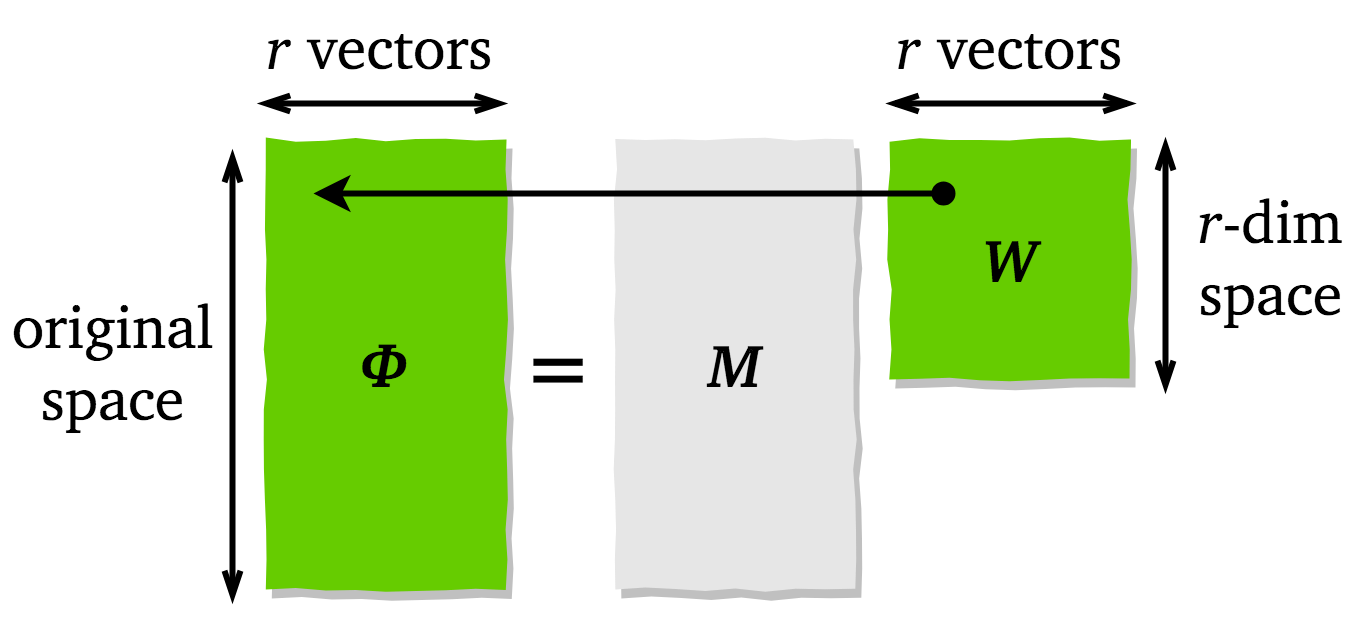
\includegraphics[width=8cm]{dmd-modes-transformation.png}
\caption{Every of the $r$ vectors in the eigenvectors matrix $\bm{W}$ gets transformed into one of the $r$ vectors in the DMD modes matrix $\bm{\Phi}$. $\bm{M}$ is the matrix associated with this transformation. We have moved from the $r$-dimensional space onto the original space.}
\label{fig:linear_system}
\end{figure}

\subsection{DMD solution}

The solution to the original dynamical system is finally computed:

\begin{equation} \label{eq:x-solution-matrix}
\vec{x}(t) = \bm{\Phi} e^{\bm{\Omega} t} \vec{b}
\end{equation}

the above equation is equivalent to:

\begin{equation} \label{eq:x-solution-summation}
\vec{x}(t)  = \sum_{k=1}^{r} \phi_k e^{\omega_k t} b_k
\end{equation}

The vector $\vec{b}$ is a vector of initial amplitudes for each mode. It is computed by projecting the initial state of the data matrix (given by $\vec{x}_1$) onto the DMD modes. This is done in order for our initial condition to be formulated in the obtained DMD basis.



\section{A broader view} \label{sec:view}

What can go different with our data sets?

\subsection{Optimized DMD}

- varying time steps

We mentioned earlier, that 

\subsection{Robust DMD}



Sparse Identification




\subsection{Multi-diagnostics DMD}

\section{Python example}



\appendix

\section{Solution to linear dynamical systems} \label{app:A}

We first recall the general solution to the differential equation:

\begin{equation} \label{eq:DE_exp}
\frac{d f(x)}{dt} = f(x)
\end{equation}

to be the exponential function: $f(x) = a \cdot e^{x}$.


In an analogous way, the general solution to the linear dynamical system of the form:

\begin{equation} \label{eq:system_linear_A}
\frac{d \vec{x}}{dt} = \bm{A} \vec{x}
\end{equation}

is:

\begin{equation} \label{eq:general_solution_A}
\vec{x} = \vec{v} e^{\bm{\lambda} t}
\end{equation}

Computing the time derivative of the eq. \ref{eq:general_solution_A} we get:

\begin{equation} \label{eq:sub1}
\frac{d \vec{x}}{dt} = \vec{v} \bm{\lambda} e^{\bm{\lambda} t}
\end{equation}

And substituting the eq. \ref{eq:general_solution_A} to eq. \ref{eq:system_linear_A} we get:

\begin{equation} \label{eq:sub2}
\frac{d \vec{x}}{dt} = \bm{A} \vec{v} e^{\bm{\lambda} t}
\end{equation}

The nontrivial solution for the equality of these two above equations is obtained when:

\begin{equation} \label{eq:eigval}
\bm{A} \vec{v} = \bm{\lambda} \vec{v} 
\end{equation}

which is the statement of eigenvalue problem.



\begin{figure}[H]
\centering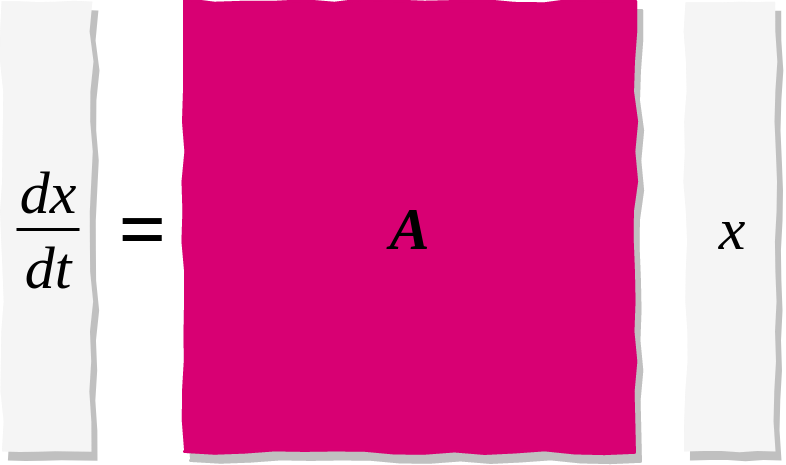
\includegraphics[width=5cm]{lin-dyn.png}
\caption{Linear dynamical system.}
\label{fig:linear_system}
\end{figure}










\section{Moore-Penrose inverse} \label{app:B}




\section{Singular Value Decomposition} \label{app:C}


\begin{figure}[H]
\centering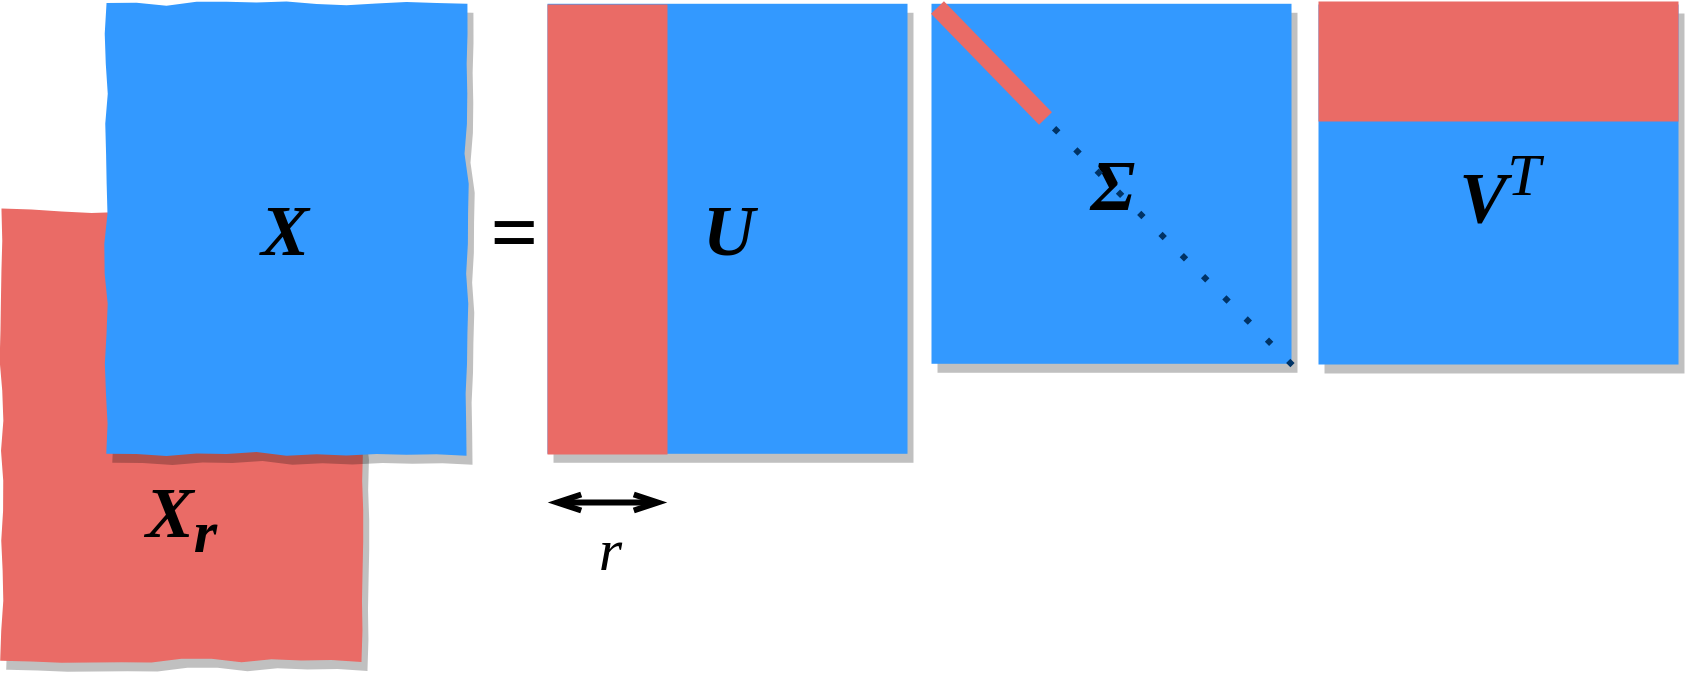
\includegraphics[width=8cm]{svd.png}
\caption{Sizes of component matrices in the Singular Value Decomposition and after rank truncation.}
\label{fig:linear_system}
\end{figure}


\thebibliography{}

\bibitem{Grosek} J. Grosek, N. Kutz, \textit{Dynamic Mode Decomposition for Real-Time Background/Foreground Separation in Video}, 2014

\bibitem{Prof_Nathan_Kutz} N. Kutz, \textit{Dynamic Mode Decomposition Theory}, an online lecture: \verb|https://youtu.be/bYfGVQ1Sg98| \label{bib:kutz_1}

\bibitem{Prof_Nathan_Kutz} N. Kutz, \textit{Dynamic Mode Decomposition Code }, an online lecture: \verb|https://youtu.be/KAau5TBU0Sc| \label{bib:kutz_2}

\bibitem{Andymation} \verb|https://www.youtube.com/watch?v=ZCCETV-8950| \label{bib:andymation}

\bibitem{Prof_Edward_Scheinerman} E. R. Scheinerman, \textit{Invitation to Dynamical Systems}

\bibitem{Prof_Gilbert_Strang} G. Strang, \textit{Introduction to Linear Algebra}, 5th edition

\bibitem{Zdybal} K. Zdybal, \textit{POD and DMD decomposition of numerical and experimental data}, von Karman Institute for Fluid Dynamics, stagiaire report 



\end{document}
